\documentclass[11pt]{article}
\usepackage{subfig}
\usepackage{color}
\usepackage{wrapfig}
\definecolor{deepblue}{rgb}{0,0,0.5}
\definecolor{deepred}{rgb}{0.6,0,0}
\definecolor{deepgreen}{rgb}{0,0.5,0}

\usepackage{listings}
\newcommand\pythonstyle{\lstset{
		language=Python,
		basicstyle=\ttm,
		otherkeywords={self},             % Add keywords here
		keywordstyle=\ttb\color{deepblue},
		emph={MyClass,__init__},          % Custom highlighting
		emphstyle=\ttb\color{deepred},    % Custom highlighting style
		stringstyle=\color{deepgreen},
		frame=tb,                         % Any extra options here
		showstringspaces=false            % 
}}
% Python environment
\lstnewenvironment{python}[1][]
{
	\pythonstyle
	\lstset{#1}
}
{}
\usepackage{geometry}
 \geometry{
 a4paper,
 left=16mm,
 top=16mm,
 right=16mm,
 bottom=16mm
 }

    \makeatletter
    \renewcommand\section{\@startsection {section}{1}{\z@}%
                                       {-3.5ex \@plus -1ex \@minus -.2ex}%
                                       {2.3ex \@plus.2ex}%
                                       {\normalfont\fontfamily{phv}\fontsize{16}{19}\bfseries}}
    \renewcommand\subsection{\@startsection{subsection}{2}{\z@}%
                                         {-3.25ex\@plus -1ex \@minus -.2ex}%
                                         {1.5ex \@plus .2ex}%
                                         {\normalfont\fontfamily{phv}\fontsize{14}{17}\bfseries}}
    \renewcommand\subsubsection{\@startsection{subsubsection}{3}{\z@}%
                                        {-3.25ex\@plus -1ex \@minus -.2ex}%
                                         {1.5ex \@plus .2ex}%
                                         {\normalfont\normalsize\fontfamily{phv}\fontsize{14}{17}\selectfont}}
    \makeatother

	\usepackage{amsmath}
	\usepackage{graphicx}
	\usepackage{enumerate}
	\usepackage{natbib} 
	\usepackage{hyperref} 
	\usepackage{booktabs}
	\usepackage{longtable}
	

	\begin{document}
		
		\def\spacingset#1{\renewcommand{\baselinestretch}%
			{#1}\small\normalsize} \spacingset{1}
		
\title{SVM, Decision Tree, Time Series Datasets}
			\author{Alireza Afzal Aghaei}
			\date{\today}
			\maketitle
			
		\bigskip
		
	\begin{abstract}
Our third exercise is about support vector machines, decision trees, random forests algorithms. There is also a Bitcoin price prediction task. This task should be done using different machine learning and deep learning models such as Ada Boost, random forests, LSTMs, etc. 
	\end{abstract}


	\spacingset{1.5} 

\section{Support Vector Machines}

1) The kernel methods are used to project the raw data into another space in which data can be modeled easier, i.e. using a linear model. The most used kernels are RBF, Polynomial, Sigmoid, Tanh and linear. The linear kernel does not transform the data while others do some projections. For example, polynomial kernels project data into a $n$ dimensional polynomial space. Among various choices of kernels, Radial Basis Functions(RBFs) are the most used ones. This kernels project data into a infinite dimensional space which is composed of all polynomial degrees from $0$ to $\infty$. So the kernel can reveals all the information which the data holds. If the data classes are nested circles, using the RBF kernels may increase the accuracy of model and reduce complexity of training phase.
\\

2,3) Various combinations of parameters are reported in table \ref{tbl:1}.
\begin{table}[]
\centering
\begin{tabular}{@{}cccccc@{}}
\toprule
\textbf{Kernel} & \textbf{C} & \textbf{Gamma (RBF)} & \textbf{Degree(Poly)} & \textbf{Test Accuracy} & \textbf{Train Accuracy} \\ \midrule
linear & 1 & - & - & 95.89 & 97.8 \\
linear & 100 & - & - & \textbf{97.05} & 99.09 \\
linear & 1000 & - & - & \textbf{97.05} & 99.69 \\
rbf & 1 & 0.1 & - & 80.97 & 99.89 \\
rbf & 1 & 0.001 & - & 72.77 & 75.63 \\
rbf & 1 & scale & - & 88.14 & 98.25 \\
rbf & 100 & 0.1 & - & 81.58 & 100.0 \\
rbf & 100 & 0.001 & - & 94.78 & 97.27 \\
rbf & 100 & scale & - & 88.84 & 100.0 \\
rbf & 1000 & 0.1 & - & 81.58 & 100.0 \\
rbf & 1000 & 0.001 & - & 95.39 & 99.4 \\
rbf & 1000 & scale & - & 88.84 & 100.0 \\
poly & 1 & - & 2 & 43.29 & 63.53 \\
poly & 1 & - & 3 & 76.08 & 95.15 \\
poly & 100 & - & 2 & 52.65 & 83.05 \\
poly & 100 & - & 3 & 74.42 & 100.0 \\
poly & 1000 & - & 2 & 55.76 & 87.55 \\
poly & 1000 & - & 3 & 74.42 & 100.0 \\ \bottomrule
\end{tabular}
\caption{Comparison of different parameters for SVM}
\label{tbl:1}
\end{table}
\\

4) Since hard margin is equivalent to a soft margin model with a very large $C$, we consider the cases $C=1000$ in the table \ref{tbl:1} as hard margin SVM.
\\

5) We have done such feature engineering tasks in the previous exercise. 
\\

6) Table \ref{tbl:1} contains these features which has been developed in the previous exercise.
\section{Decision Trees}
7) ID3 (Iterative Dichotomiser 3) was developed in 1986 by Ross Quinlan. The algorithm creates a multiway tree, finding for each node (i.e. in a greedy manner) the categorical feature that will yield the largest information gain for categorical targets. Trees are grown to their maximum size and then a pruning step is usually applied to improve the ability of the tree to generalise to unseen data. 
C4.5 is the successor to ID3 and removed the restriction that features must be categorical by dynamically defining a discrete attribute (based on numerical variables) that partitions the continuous attribute value into a discrete set of intervals. C4.5 converts the trained trees (i.e. the output of the ID3 algorithm) into sets of if-then rules. This accuracy of each rule is then evaluated to determine the order in which they should be applied. Pruning is done by removing a rule’s precondition if the accuracy of the rule improves without it.
CART (Classification and Regression Trees) is very similar to C4.5, but it differs in that it supports numerical target variables (regression) and does not compute rule sets. CART constructs binary trees using the feature and threshold that yields the largest information gain at each node.

For a complete comparison of ID3, C4.5 and Cart, we refer the reader to \href{https://link.springer.com/chapter/10.1007/978-81-322-2205-7_51}{this link}.
\\
8) Our tests shows that the decision trees does not useful for this type of data. In the table \ref{tbl:2} we reported train \& test accuracy for different combinations of parameters.
\begin{table}[]
\centering
\begin{tabular}{@{}ccccc@{}}
\toprule
\textbf{Criterion} & \textbf{Max depth} & \textbf{Splitter} & \textbf{Test Accuracy} & \textbf{Train Accuracy} \\ \midrule
 \\ \midrule
gini & 5 & random & 72.47 & 74.91 \\
gini & 5 & best & 82.17 & 88.11 \\
gini & 10 & random & 81.58 & 95.55 \\
gini & 10 & best & 83.28 & 99.32 \\
gini & 15 & random & 81.43 & 99.95 \\
gini & 15 & best & 81.93 & 99.99 \\
gini & 20 & random & 81.38 & 100.0 \\
gini & 20 & best & 82.33 & 100.0 \\
entropy & 5 & random & 75.83 & 76.53 \\
entropy & 5 & best & 81.98 & 87.57 \\
entropy & 10 & random & 83.38 & 97.16 \\
entropy & 10 & best & \textbf{84.98} & 99.86 \\
entropy & 15 & random & 81.63 & 99.95 \\
entropy & 15 & best & 84.68 & 100.0 \\
entropy & 20 & random & 82.43 & 100.0 \\
entropy & 20 & best & 84.08 & 100.0 \\ \bottomrule
\end{tabular}
\caption{Comparison of different parameters of decision tree}
\label{tbl:2}
\end{table}
\\
9) As you can see in the \ref{tbl:2}, Increasing the depth of the tree usually leads to overfitting. 
\\
10) As the name implies, pruning involves cutting back the tree. After a tree has been built (and in the absence of early stopping discussed below) it may be overfitted. The CART algorithm will repeatedly partition data into smaller and smaller subsets until those final subsets are homogeneous in terms of the outcome variable. In practice this often means that the final subsets (known as the leaves of the tree) each consist of only one or a few data points. The tree has learned the data exactly, but a new data point that differs very slightly might not be predicted well.
\\
12) See table \ref{tbl:3} for detailed comparison.
\begin{table}[]
\centering
\begin{tabular}{@{}ccccc@{}}
\toprule
\textbf{Criterion} & \textbf{Max depth} & \textbf{\# of estimators} & \textbf{Test Accuracy} & \textbf{Train Accuracy} \\ \midrule
gini & 5 & 10 & 70.27 & 82.93 \\
gini & 5 & 100 & 83.48 & 92.3 \\
gini & 10 & 10 & 77.58 & 98.54 \\
gini & 10 & 100 & 87.39 & 99.96 \\
gini & 15 & 10 & 79.73 & 99.7 \\
gini & 15 & 100 & 88.19 & 100.0 \\
gini & 20 & 10 & 79.73 & 99.7 \\
gini & 20 & 100 & 88.53 & 100.0 \\
entropy & 5 & 10 & 75.48 & 86.32 \\
entropy & 5 & 100 & 83.13 & 90.97 \\
entropy & 10 & 10 & 81.17 & 98.82 \\
entropy & 10 & 100 & 88.29 & 100.0 \\
entropy & 15 & 10 & 79.93 & 99.52 \\
entropy & 15 & 100 & 88.09 & 100.0 \\
entropy & 20 & 10 & 80.03 & 99.64 \\
entropy & 20 & 100 & \textbf{88.94} & 100.0 \\ \bottomrule
\end{tabular}
\caption{Comparison of different parameters of random forests}
\label{tbl:3}
\end{table}
\\
13) Because of the great interpretation of decision trees, they are used to explain the model to those who do not familiar with machine learning methods. For example see figure \ref{fig:1} for a detailed interpretation of decision tree for mobile price classification dataset.
\begin{figure}
    \centering
    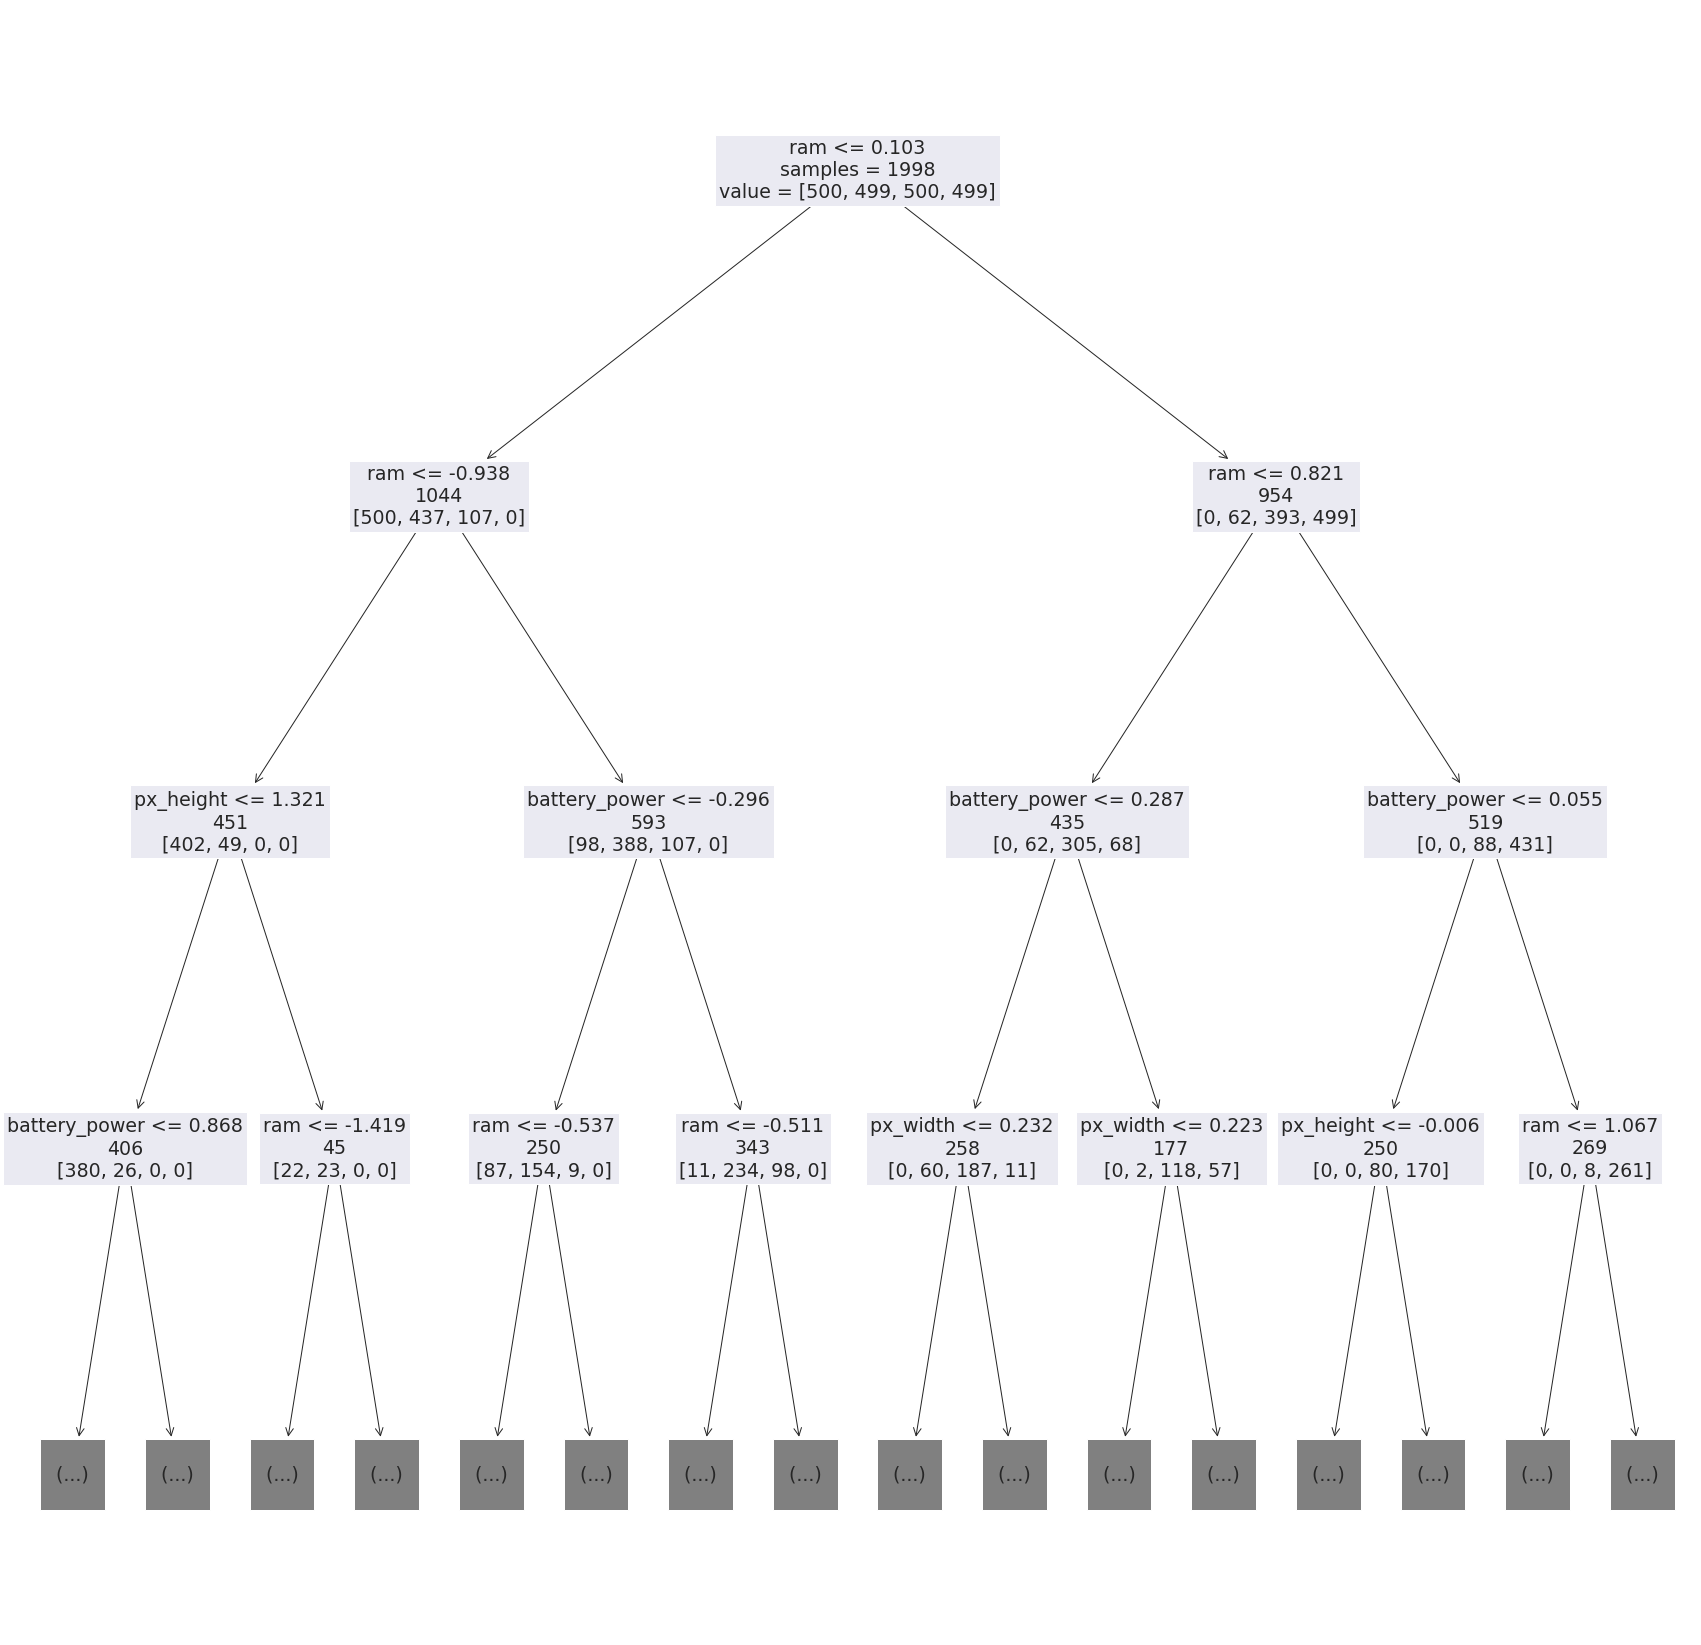
\includegraphics[width=1\textwidth]{tree.png}
    \caption{Decision tree visualization}
    \label{fig:1}
\end{figure}
15) In order to use ID3 or C4.5 decision trees time series classification, Waleed Kadous has proposed two different approaches (\href{https://www.quora.com/How-can-ID3-or-C4-5-decision-trees-be-used-for-time-series-classification}{reference}):
\begin{itemize}
\item Divide each time series (regardless of length) into a number of windows (say 5 -- eg. if training example A is 45 samples long, divide it into times 1-9,10-18, etc. Training example B is 60 samples long, divide it into 1-12 etc). Compute statistics, say the mean and gradient, for each of the windows. Feed this into a learning like C4.5 or ID3. You can determine the optimal number of windows for a data set by cross-validation.

Upsides: This worked surprisingly well for such a simple algorithm (testing on sign language and ECGs). This was meant to be my "baseline" learner, but I had unwittingly set myself a high bar.

Downsides: the learnt concepts are not very comprehensible. Works well for "trending" data, does not work well for data with rapid changes, or where events happen at different times.

\item Create "primitives" that you might look for in the data (e.g. peaks, plateaus) etc that can be characterized by parameters (e.g. peak height, plateau level). Cluster these primitives to find templates. For each time series, check for the presence/absence of these templates to construct a feature. Then feed this into C4.5.

Upsides: Allows you to include background knowledge via primitives. Produces semi-comprehensible descriptions (e.g. if you have a peak early, then a plateau it is class A).
\end{itemize}

\section{Time Series Datasets}
16) As the question asked, we fetched the bitcoin price from 01-01-2010 until 01-05-2021 in a daily format. But the downloaded data starts from 18-07-2010. Anyway, we split the data into train and test sets. The training data covers the 18-07-2010 to 01-01-2020 and the test set contains the bitcoin price from 02-01-2020 till 01-05-2021. 


\begin{quote}
Bitcoin was trading around \$38,074, according to Coindesk, when at about 3:42 p.m. ET Musk posted on Twitter: “Spoke with North American Bitcoin miners. They committed to publish current \& planned renewable usage \& to ask miners WW to do so. Potentially promising.”

Within minutes, the price had shot up to more than \$39,500. Overall, the coin is up more than 17\% in the last 24 hours.
\end{quote}
Obviously, the bitcoin price is highly affected by media news.  A novel technique we have used in this section, is to collect the bitcoin news published on Hacker News. This data was collected using BigQuery API. We counted the number of published news everyday during 18-07-2010 until 01-05-2021. The table \ref{tbl:4} shows some samples of the data.

\begin{table}[]
\centering
\begin{tabular}{@{}cccc@{}}
\toprule
\textbf{Date} & \textbf{Price} & \textbf{log(Price)} & \textbf{Num News} \\ \midrule
2012-11-02 & 10.5 & 2.351375 & 0 \\
2013-04-17 & 93.1 & 4.533674 & 19 \\
2014-01-01 & 815.9 & 6.704292 & 7 \\
2014-07-06 & 626.7 & 6.440468 & 0 \\
2015-05-19 & 232.0 & 5.446737 & 12 \\
2016-10-02 & 610.7 & 6.414606 & 1 \\
2017-12-09 & 14843.4 & 9.605311 & 28 \\
2018-11-02 & 6424.7 & 8.767905 & 10 \\
2020-04-28 & 7746.9 & 8.955048 & 4 \\ \bottomrule
\end{tabular}
\caption{Some rows of our BTC dataset}
\label{tbl:4}
\end{table}

\subsection{Facebook's Prophet}
In order to use fbprophet package, we first transformed the BTC price into logarithmic scale. The "Num News" feature is dropped in this case. The parameters of the model are as follows:

\begin{python}
model = Prophet(
          changepoint_range=0.99, 
          yearly_seasonality='auto', 
          weekly_seasonality=False, 
          daily_seasonality=True,
          seasonality_mode='multiplicative',
          seasonality_prior_scale=.2,    
          n_changepoints=15
    )
\end{python}
Figure \ref{fig:2} shows the prediction of Facebook's prophet.

\begin{figure}
    \centering
    \subfloat[\centering Logarithmic Scale]{{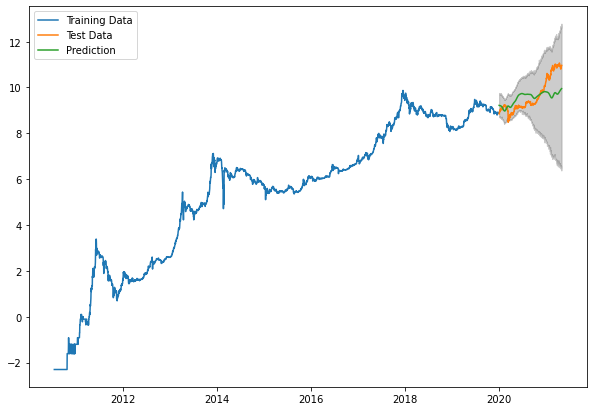
\includegraphics[width=.49\textwidth]{prophet01.png} }}%
    \subfloat[\centering Real Scale]{{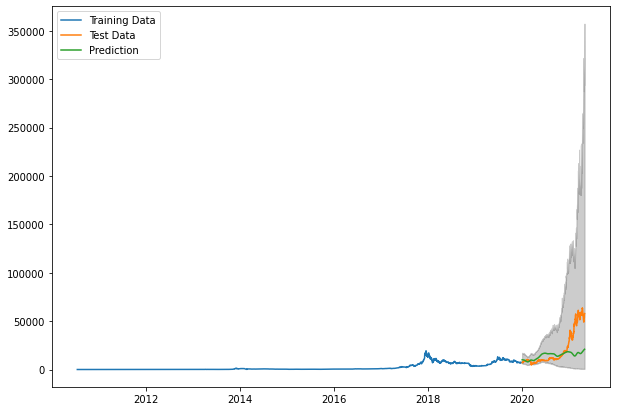
\includegraphics[width=.5\textwidth]{prophet02.png} }}%
    
    \caption{Facebook's prophet prediction of Bitcoin price}
    \label{fig:2}
\end{figure}

\subsection{LSTM-1}
In this case we only use the price feature. for each day we use the current price as input data and the tomorrow price as the target variable. Again, we use the logarithmic scale here. The architecture of out model is:

\begin{python}
regressor = Sequential()
regressor.add(LSTM(units = 10, activation = 'sigmoid', input_shape=(None, 1)))
regressor.add(Dense(units = 5))
regressor.add(Dense(units = 1))
\end{python}

In the figure \ref{fig:3} we have plotted the excellent prediction of out LSTM model.

\begin{figure}
    \centering
    \subfloat[\centering Logarithmic Scale]{{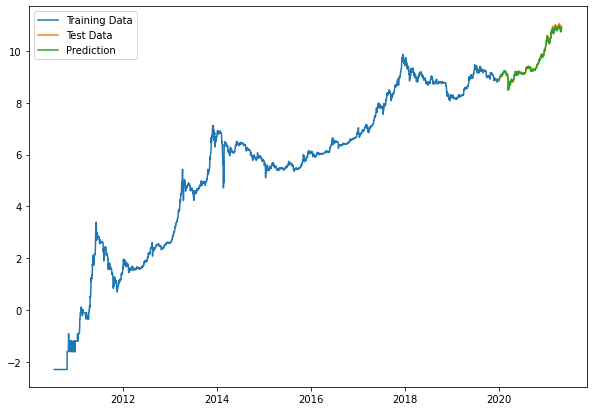
\includegraphics[width=.49\textwidth]{lstm01.png} }}
    \subfloat[\centering Real Scale]{{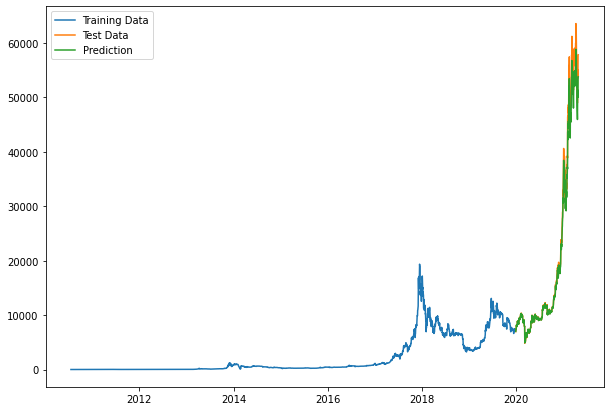
\includegraphics[width=.50\textwidth]{lstm02.png} }}%
    
    \caption{LSTM prediction of Bitcoin price}
    \label{fig:3}
\end{figure}

\begin{wrapfigure}{o}{9cm}
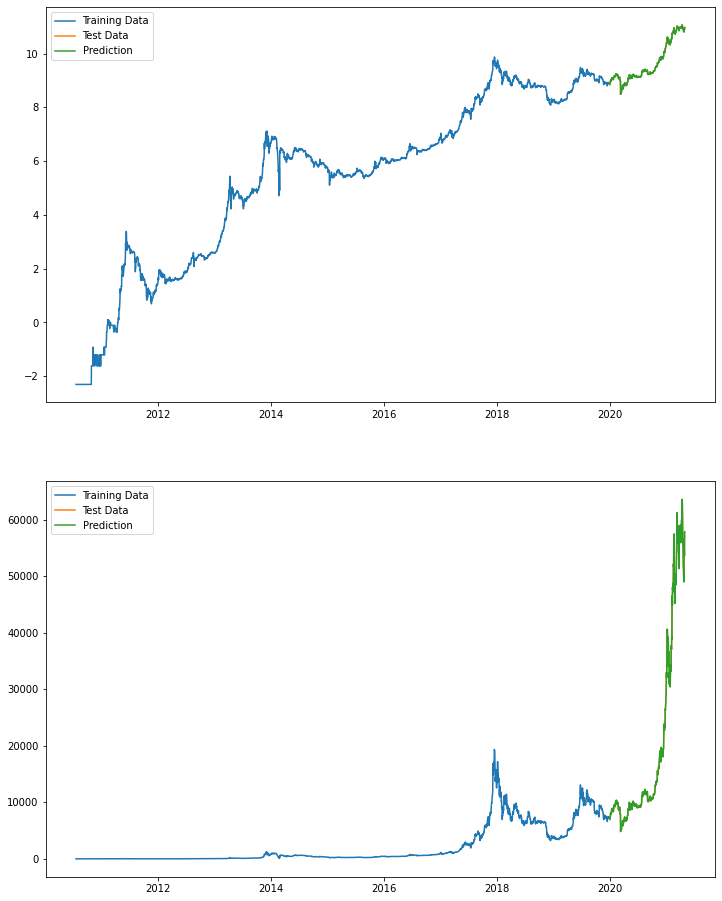
\includegraphics[width=8.5cm, height=11.5cm]{mlp.png}
    \caption{MLP prediction of Bitcoin price}
    \label{fig:4}
\end{wrapfigure} 

\subsection{LSTM-2}
The previous model just uses the price feature for both input and output training data. In this case, we use price and news count as input data and the price as target variable. Using this feature we can see that the accuracy of prediction increases. The results are reported in the comparison section. 



\subsection{LSTM-3}

The previous model reshapes the data points into the shape (-1, 2, 1) in which -1 means the number of samples. In this case the input shape of LSTM layer was (None, 1). 

In this model we reshape the data to (-1, 1, 2) which means the LSTM input shape is (None,2). Using this model increases the accuracy a from 76\% to 88\%. See comparison section for more details. 

\subsection{MLP}
In this case we have used Multi Layer Perceptron model to predict BTC price. The model contains a hidden layer with 3 number of neurons. This model has great prediction. It reached the 100\% accuracy and the RMSE 12\$ on the test set. See the prediction plot in figure \ref{fig:4}.

\subsection{AdaBoost}
We used Adaboost with DecisionTree (DT) and Linear Regression (LR) models. 

\begin{figure}
    \centering
    \subfloat[\centering Decision Tree]{{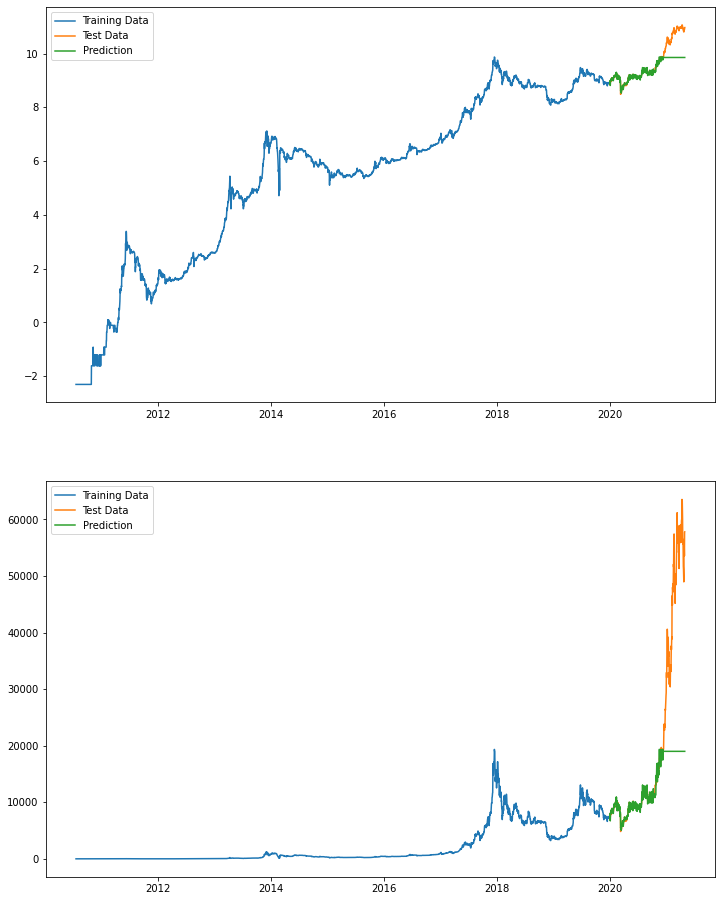
\includegraphics[width=.49\textwidth]{adaboost01.png} }}
    \subfloat[\centering Linear Regression]{{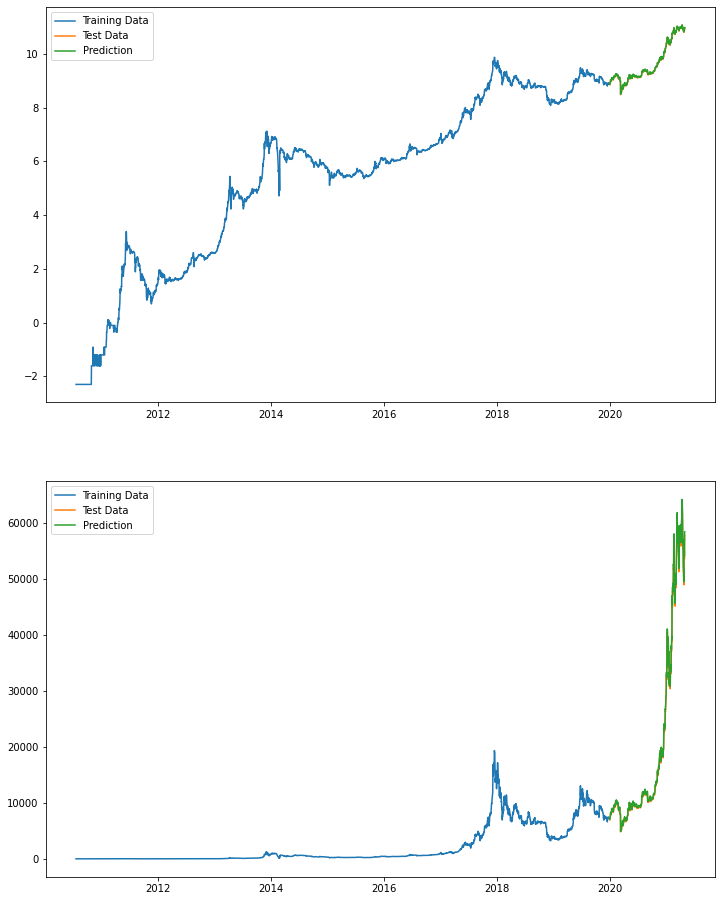
\includegraphics[width=.50\textwidth]{adaboost02.png} }}%
    \caption{Adaboost prediction of Bitcoin price}
    \label{fig:5}
\end{figure}
\subsection{Comparison}
See the comparison of the aforementioned methods in the table \ref{tbl:5}. It is seen that the MLP model has the best prediction RMSE and Accuracy.
\begin{table}[]
\centering
\begin{tabular}{@{}llll@{}}
\textbf{Model} & \textbf{RMSE (log)} & \textbf{RMSE (real)} & \textbf{Accuracy (real)} \\ \midrule
fbProphet & 0.6063 & 16774.3388 & 0.06\% \\
LSTM-1 & 0.0412 & 1993.8161 & 75.51\% \\
LSTM-2 & 0.0510 & 2310.2968 & 76.13\% \\
LSTM-3 & 0.0286 & 1370.1983 & 88.47\% \\
MLP & \textbf{0.0009} & \textbf{12.3681} & \textbf{100\%} \\
Adaboost(DT) & 0.4724 & 15484.2455 & 51.85\% \\
Adaboost(LR) & 0.01110 & 226.1971 & \textbf{100\%} \\
Random Forest & 0.47651 & 15571.2249 & 61.93\% \\ \bottomrule
\end{tabular}
\caption{Comparison of different methods for predicting bitcoin price}
\label{tbl:5}
\end{table}

\section{The unknown Dataset!}
26) In this question, a big dataset was given. Since the real value of the test data given in dataset (named tournament\_data) we drop this in our case, and split the train data into two disjoint train and test sets.

The data has 5 different classes: $0, 0.25, 0.5, 0.75, 1$. The Question does not specified the type of problem. If the values are ordered or the rational values such as $.24, 0.78$, etc. are meaningful, we should use regression models. Otherwise it is better to use classification methods.

The first challenge in this case, is the size of data. Since the number of samples are more than 500,000 we can not use arbitrary machine learning models. For example Support Vector Machines (SVMs) create a $500,000\times 500,000$ matrix of data which is impossible to save it RAM. Additionally, solving a Quadratic Program with this size is not computationally efficient. For this case it is better to use efficient methods like Decision Trees or Linear Regression models.

The next challenge is the data imbalance. As you can see in the table \ref{tbl:6}, nearly half of the data has class value $0.5$. Actually the target variable for this data has normal distribution! If we use a non smart regression model, it learns to map every input to $0.5$ in this model the empirical error will be minimized.

To solve this problem we have used two different methods. In the first method we considered the problem as a imbalanced classification task, and used class weights parameter of sklearn methods to balance the data.

The Next method is to drop some data! To do so, we only hold $25016$ sample for each class. This creates a dataset with the size of $125080$ samples. Now, we can run various regression and classification methods on this dataset.

To simulate these data, we have used different methods such as XGBoost Regression and classification, Linear and Logistic regression, Decision Tree and Random forests and SGD Classifier and regressor methods. 

The best obtained mean absolute error for these models are about $0.14$. Actually the models map the input test data to $0.5$. We have used PCA dimensionally reduction method and a simple single hidden layer perceptron neural network, but the results are same!
\begin{table}[]
\centering
\begin{tabular}{@{}cc@{}}
\toprule
Target & Value Counts \\ \midrule
0.50 & 251677 \\
0.25 & 100053 \\
0.75 & 100045 \\
1.00 & 25017 \\
0.00 & 25016 \\ \bottomrule
\end{tabular}
\caption{The target value counts of the unknown dataset!}
\label{tbl:6}
\end{table}
\end{document}